% =====================================================================
%  第 4 节  用一次量子化证明 A∞ 关系式（原书 p.20–25）
%  含 4.1、4.2、式 (48)–(56)、例 6、例 7、注 4.1、图 11、图 12
% =====================================================================
\section{用一次量子化证明 $\Ainf$ 关系式}\label{sec:4}

\begin{takeaway}
\begin{itemize}
  \item \textbf{物理图像}：把 $X$ 上单粒子的超量子力学放到树上。每条边是一段“时间”，超传播子 $U(t,\mathrm{d}t)=e^{-tH-\mathrm{d}t\,G}$ 沿边传播态；叶子是入态（$F_a-F_b$ 的 Lefschetz thimble 上的 delta 形式），2 价顶点是“乘以链 $Z$ 上 delta 形式”的插入算子，3 价顶点按 $(a,b)\times(b,c)=(a,c)$ 把颜色接起来。
  \item \textbf{数学工具}：度量树模空间 $MT_{a_1,\dots,a_r;k_1,\dots,k_r}$；取值于 $\mathrm{Hom}$ 空间的微分形式 $I$；Morse 收缩的三元组 $(i,p,K)$ 与超传播子在边趋于无穷时的行为 $U(+\infty)=i\circ p$；模空间上的 Stokes 定理。
  \item \textbf{主要结论}：$I$ 满足 $(\mathrm{d}_{MT}+Q)I=0$，在红外边界上分解，其周期恰为复合映射 $m$。把这条闭性等式在模空间上积分，两端分别给出 $Qm$ 与边界层片之和；五类层片中三类相消、两类保留，合起来正是 $A_\infty$ 关系式~\eqref{eq:7}。
\end{itemize}
\end{takeaway}

% [Tutor Note: 本节是第~\ref{sec:3} 节的“对偶”版本。第~\ref{sec:3} 节走二次量子化：把 $X$ 上的 BF 理论作纤维 BV 积分，树是 Feynman 图。本节走一次量子化：树本身是单粒子超量子力学的“时间轴分叉”，模空间 $MT$ 只负责记录各边长度。两条路线给出同一批复合映射，但本节只需 $MT$ 上一个闭形式加 Stokes 定理。]

\subsection{树上高阶拓扑量子力学的进路：思路}\label{sec:4.1}

\begin{takeaway}
\begin{itemize}
  \item \textbf{物理图像}：单粒子的超量子力学以 $Q=\mathrm{d}$ 为奇幂零对称性，取 $G=\iota_{v_{ab}}$、$H=[Q,G]=L_{v_{ab}}$：$G$ 降一次、$H$ 保持次数。树的分叉由 3 价顶点按颜色规则实现，叶子与链则作为入态或插入算子。
  \item \textbf{数学工具}：类型为 $(a,b)$ 的粒子、态空间 $\Omega^\bullet(X)$、超传播子 $U(t,\mathrm{d}t)$、带度量且顶点价数为 1、2、3 的树。
  \item \textbf{主要结论}：由 $U$ 的展开得到边长度空间上的闭微分形式；它在某条边趋于无穷时分解。于是沿红外边界积分，就得到 $A_\infty$ 关系式的粗略论证；细节见第~\ref{sec:4.2} 节。
\end{itemize}
\end{takeaway}

我们考虑树上的高阶拓扑量子力学，给出范畴 $\mathbb{F}$ 中 $A_\infty$ 关系式~\eqref{eq:7} 的第二个证明。\footnote{高阶拓扑量子力学（higher topological quantum mechanics，HTQM）的设定见 \cite{losev,losevpolyubin}。粗略地说，HTQM 就是度量树模空间上的一个闭微分形式，它在任何一条边变得无限长时分解。于是由模空间上的 Stokes 定理，该形式的各个周期之间出现二次关系。这套框架本质上是一个链层面、一维的上同调场论，见 \cite{kontsevichmanin}。}

普通量子力学由粒子的态空间与 Hamilton 量描述。我们考虑类型为 $(a,b)$（$a\neq b$）的粒子，其态空间始终取流形 $X$ 上微分形式构成的空间。Hamilton 量取为沿 $F_a-F_b$ 的梯度向量场 $v_{ab}$ 的 Lie 导数 $L_{v_{ab}}$。这类 Hamilton 量关于一个奇、幂零的对称性 $Q$ 是正合的：
\[
  Q=\mathrm{d},\qquad G=\iota_{v_{ab}},\qquad H=[Q,G]=L_{v_{ab}}.
\]

我们考虑带度量（即各边长度）的树，其顶点的价数为 1、2、3。

1 价顶点是一个态：对 $(a,b)$-粒子，我们把这个态取为函数 $F_a-F_b$ 的临界点 $P_{ab}$ 所对应的 Lefschetz thimble（不稳定流形）上的 delta 形式。2 价顶点不过是态空间中的一个算子，即乘以链 $Z$ 上 delta 形式的算子。3 价顶点是微分形式的乘法，并配上规则
\[
  (a,b)\times(b,c)=(a,c),
\]
其余情形取零。我们用超传播子（又称演化算子）
\begin{equation}\tag{48}\label{eq:48}
  U(t,\mathrm{d}t)=\exp(-tH-\mathrm{d}t\,G)
\end{equation}
来构造边长度空间上的微分形式。这个对象已在上文讨论 Morse 收缩时出现过，见式~\eqref{eq:9}。

% [Tutor Note: 式 (48) 与式 (9) 是同一个算子：式 (9) 把它写成 $e^{-tL_v}(1-\mathrm{d}t\,\iota_v)$。因为 $(\mathrm{d}t\,\iota_v)^2=0$ 且 $[L_v,\iota_v]=0$，指数可以拆开，两种写法一致。关键在于每次出现 $\mathrm{d}t$ 必同时出现一个 $\iota_v$，这条“捆绑”是全节次数计数的起点。]

把该传播子展开，就得到边长度空间上的一个微分形式。当某条边的长度趋于无穷时，这个形式分解。

论证的粗略思路如下（正确的版本见下文）。按上述方式构造的微分形式是闭的。因此可以沿红外边界（即某条边的长度等于无穷时）对它积分。利用分解性质，就得到各长度空间上的积分之间所期望的二次关系，而这些关系恰是我们要证明的 $A_\infty$ 关系式~\eqref{eq:7}。

% [Tutor Note: 这条“闭形式加边界分解”的论证与上同调场论中 WDVV 方程的证明同构：那里模空间是带四个标记点的球面模空间（复一维），边界是三个点；这里模空间是一维的树模空间，边界只由 $t\to0$ 与 $t\to+\infty$ 组成。两者都归结为一组二次关系，一维版本就是 $\Ainf$ 关系式。见 \cite{losev,kontsevichmanin}。]

\subsection{更多细节}\label{sec:4.2}

\begin{takeaway}
\begin{itemize}
  \item \textbf{物理图像}：一个胞腔由树的组合型与各内部边长 $t,t',t''$ 的正实数值决定；边长为零等于把该边收缩，边长趋于无穷则是红外边界。$I$ 是把 $U$ 逐边装配、再在 2 价顶点插入链得到的微分形式。
  \item \textbf{数学工具}：$MT_{a_1,\dots,a_r;k_1,\dots,k_r}$、形式 $I$ 及其三条性质（闭性、红外分解、周期）、式~\eqref{eq:14} 的 $(\mathrm{d}_t+Q)$-闭性、$\mathrm{d}t$-次数计数。
  \item \textbf{主要结论}：由 $(\mathrm{d}_{MT}+Q)I=0$ 与 Stokes 定理得式~\eqref{eq:55}；左端按边界层片分成五类，(a)(b)(c) 三类两两相消，(d)(e) 两类保留，与右端的 $Qm$ 合起来正好是 $A_\infty$ 关系式。例~\ref{ex:7} 与图~\ref{fig:12} 给出具体核对。
\end{itemize}
\end{takeaway}

固定一列“颜色” $a_1,\dots,a_r\in\{1,\dots,N\}$，满足对一切 $i$ 有 $a_i\neq a_{i+1}$；再固定一列整数 $k_1,\dots,k_r\ge0$。我们考虑度量树的模空间 $MT_{a_1,\dots,a_r;k_1,\dots,k_r}$：它是带 $r-1$ 个入向 1 价顶点（叶子）与一个出向顶点（根）的有根带状树。带的侧边（border）标有颜色 $a_1,\dots,a_r$，从根出发逆时针行进时以 $a_1$ 起始，并在遇到的第 $i$ 个 1 价顶点处由 $a_i$ 换成 $a_{i+1}$。树上还有 $k_i$ 个颜色为 $a_i$ 的 2 价顶点，它们分布在与第 $i$ 条侧边相邻的那些边上。于是，每条边与每个 1 价顶点都带双色 $(a,b)$（$a\neq b$），而每个 2 价顶点带单一颜色 $a$，并且只能出现在双色为 $(a,b)$ 或 $(b,a)$ 的线上，其中 $b$ 是另一个颜色。

我们给内部边（即不与 1 价顶点相邻的边；与 1 价顶点相邻的边一律理解为长度为 $+\infty$）配上长度 $t_j>0$；极限 $t_j\to0$ 理解为把一条边收缩。于是
\[
  MT=\bigcup \mathbb R_+^{\#\mathrm{int.}\ \mathrm{edges}}/\sim,
\]
其中并取遍类型为 $(a_1,\dots,a_r;k_1,\dots,k_r)$ 的树的各个组合型，而 $\sim$ 表示把“有一条长度为 0 的边”的树与“该边已收缩”的树等同起来。

% [Tutor Note: “内部边”不含紧挨 1 价顶点的边，那类边长度恒为 $+\infty$。因此 $\dim MT$ 等于内部边条数，图~\ref{fig:11} 的三棵树各有 $t$、$t'$、$t''$ 三条内部边，都是 3 维胞腔。$t\to0$ 是 UV 边界（收缩），$t\to+\infty$ 是 IR 边界（分解），两者在式~\eqref{eq:55} 的左端分别对应 (a)–(d) 类与 (e) 类层片。]

\begin{figure}[htbp]
  \centering
  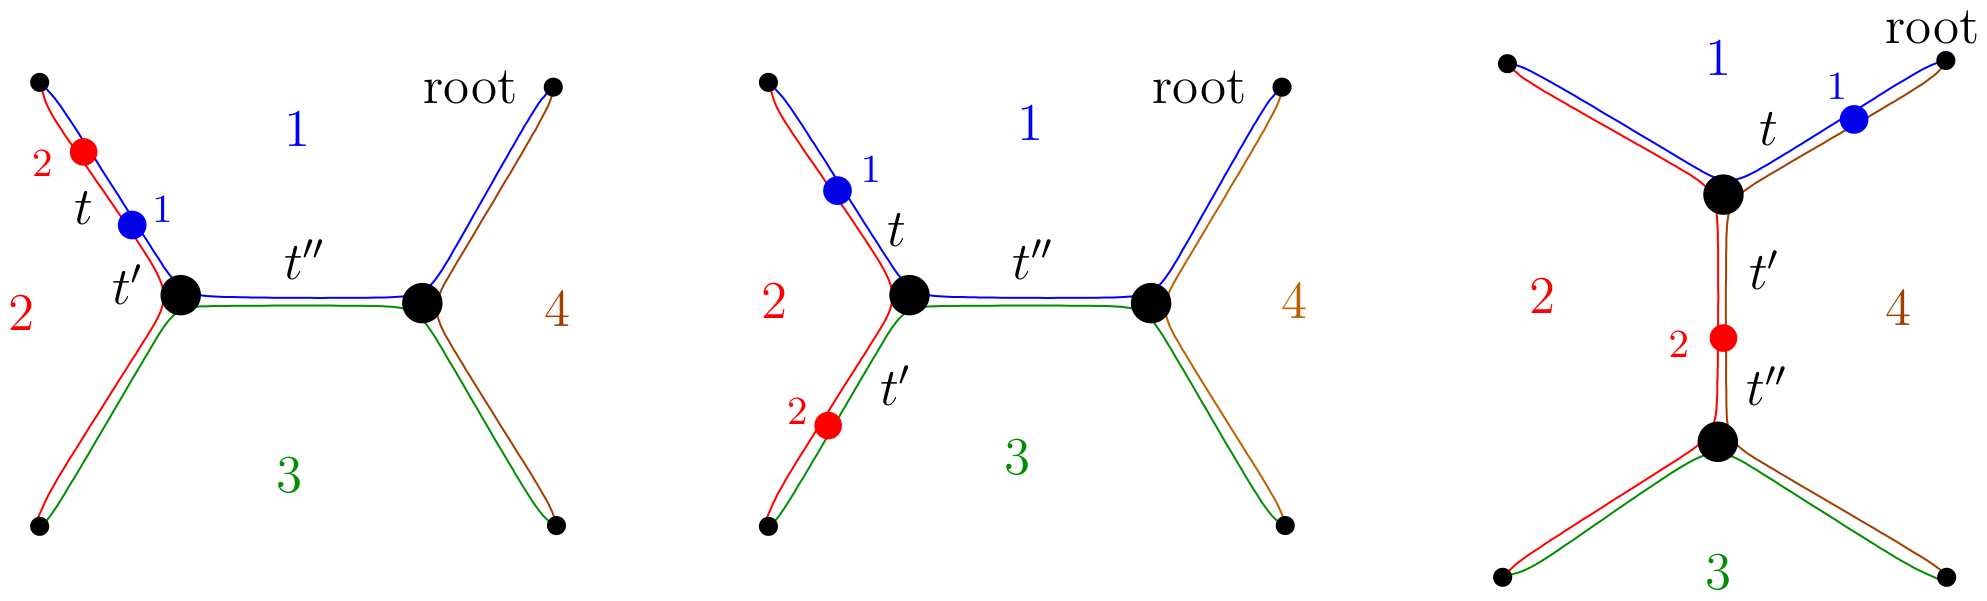
\includegraphics[width=\linewidth]{fig11.png}
  \caption{$MT_{1,2,3,4;1,1,0,0}$ 的三个最高维胞腔。（原书 p.22）}
  \label{fig:11}
\end{figure}

上述构造给出树模空间上的一个微分形式（在 \cite{losev} 的术语中称为前振幅，pre-amplitude）：
\begin{equation}\tag{49}\label{eq:49}
\begin{aligned}
I\in{}&\Omega^\bullet(MT_{a_1,\dots,a_r;k_1,\dots,k_r})\otimes\\
&\otimes\mathrm{Hom}\bigl(\Mor^{\otimes k_1}_{a_1,a_1}\otimes\Mor_{a_1,a_2}\otimes\cdots\otimes\Mor_{a_{r-1},a_r}\otimes\Mor^{\otimes k_r}_{a_r,a_r},\ \Mor_{a_1,a_r}\bigr).
\end{aligned}
\end{equation}
这里我们简记 $\Mor_{a,b}:=\mathbb R\otimes\Mor(F_a,F_b)$，即 $\mathbb{F}$ 中的态射空间与 $\mathbb R$ 的张量积。

% [Tutor Note: 原文 (49) 在两行的行末与行首各印了一个 $\otimes$，照排后出现两个张量积符号，这是排版残留，译文照印未改。另注意输入顺序与式 (3) 一致：先 $\Mor_{a_1,a_1}^{\otimes k_1}$、再 $\Mor_{a_1,a_2}$，例 6 的排法即由此而定；次序写反则 $\int_{MT}I=m$ 不成立。]

\begin{thmenv}{例}{6}\label{ex:6}
例如，对图~\ref{fig:11} 中间那棵树，有
\[
  I(t,\mathrm{d}t,t',\mathrm{d}t',t'',\mathrm{d}t'')(Z_1,[P_{12}],Z_2,[P_{23}],[P_{34}])=\sum_{P_{14}\in\mathrm{Crit}(F_1-F_4)}\bar I\cdot[P_{14}],
\]
其中
\begin{equation}\tag{50}\label{eq:50}
\begin{aligned}
\bar I(t,\mathrm{d}t,t',\mathrm{d}t',t'',\mathrm{d}t'')&=\int_X\delta_{\mathrm{Stab}P_{14}}\wedge\\
&\quad\wedge U_{F_1-F_3}(t'',\mathrm{d}t'')\Bigl(U_{F_1-F_2}(t,\mathrm{d}t)(\delta_{Z_1}\wedge\delta_{\mathrm{Unstab}P_{12}})\\
&\qquad\wedge U_{F_2-F_3}(t',\mathrm{d}t')(\delta_{Z_2}\wedge\delta_{\mathrm{Unstab}P_{23}})\Bigr)\\
&\quad\wedge\delta_{\mathrm{Unstab}P_{34}}.
\end{aligned}
\end{equation}
\end{thmenv}

这里 $\int_X\delta_{\mathrm{Stab}P_{14}}\wedge\cdots$ 是根（“出态”）的贡献。记号 $U_{F_a-F_b}$ 指 $F_a-F_b$ 的梯度向量场所对应的超传播子~\eqref{eq:48}。\footnote{注意，(50) 是式~\eqref{eq:29} 中 $\int_{\mathbb R_+^E}$ 的被积式——取对应图~\ref{fig:11} 中间那棵组合树的项——，其中对 $X^{V\setminus\{q\}}$ 的积分已经算掉；这里 $q$ 是由一条边与根相连的顶点（本例中为右侧的 3 价顶点）。}

% [Tutor Note: (50) 的次数核对法：$U=e^{-tH}(1-\mathrm{d}t\,G)$ 中 $\mathrm{d}t$ 与 $G=\iota_v$ 成对出现，每对净次数为 0，但使 $X$ 方向的形式次数降 1。要对 $X$ 与 $MT$ 同时取顶次项，需三条内部边各取一个 $\mathrm{d}t$（凑出 $\mathrm{d}t\wedge\mathrm{d}t'\wedge\mathrm{d}t''$），且 $\delta_{\mathrm{Stab}P}$、$\delta_{\mathrm{Unstab}P}$、$\delta_Z$ 的次数之和（分别为 $P$ 的指标、$P$ 的余指标、链的余维数）等于 $\dim X+3$。]

\begin{thmenv}{注}{4.1}\label{rem:4.1}
为解析上的方便——若希望入态是相应“态的态空间”中的元素（而不是极限点）——不妨把 delta 形式 $\delta_{\mathrm{Unstab}P}$ 换成它的 $\epsilon$ 光滑化版本 $\delta^{\epsilon}_{\mathrm{Unstab}P}$（同时在 2 价顶点处把正规化 $\delta_Z$ 换成 $\delta^{\epsilon}_Z$），最后在 $I$ 的表达式中取极限 $\epsilon\to0$。
\end{thmenv}

% [Tutor Note: 原文此处印作 “the respective states of states”，疑为 spaces of states 之笔误。译文照印并加引号，读者按“态空间”理解即可。之所以要光滑化：$\delta_{\mathrm{Unstab}P}$ 是分布形式，两个分布形式相乘没有定义，换成 $\delta^\epsilon$ 后所有运算都在光滑形式内完成，最后再取 $\epsilon\to0$。]

形式 $I$ 有三条关键性质。

\begin{enumerate}
  \item[(i)] \textbf{闭性.}\quad 有
  \begin{equation}\tag{51}\label{eq:51}
    (\mathrm{d}_{MT}+Q)I=0,
  \end{equation}
  其中 $\mathrm{d}_{MT}$ 是树模空间上的 de Rham 微分，$Q$ 按导子作用：它在式~\eqref{eq:49} 的每个态射空间上取相应的微分——在 $\Mor(F_a,F_b)$（$a\neq b$）上取 Morse 微分 $\mathrm{d}_{\mathrm{Morse}}$，在奇异链 $\Mor(F_a,F_a)$ 上取边界算子。式~\eqref{eq:51} 成立的原因是：用来构造 $I$ 的超传播子 $U(t,\mathrm{d}t)$ 是 $(\mathrm{d}_t+Q)$-闭的，见式~\eqref{eq:14}。

  % [Tutor Note: 这里的 $Q$ 要读成作用在算符上的分次交换子 $[\mathrm{d}_X,\cdot]$：在微分形式上它就是外微分 $\mathrm{d}$（即第 4.1 节开头的 $Q=\mathrm{d}$），在算符上则是 $[Q,\cdot]$。式 (14) 的 $(\mathrm{d}_t+[\mathrm{d}_X,-])U=0$ 与 (51) 是同一件事。]

  \item[(ii)] \textbf{在红外边界上的分解.}\quad 若图中某条边的长度变为 $+\infty$，则 $I$ 分解。模空间 $MT$ 的红外边界形如 $\bigcup_{i<j}\partial^{IR}_{ij}MT$，其中
  \begin{equation}\tag{52}\label{eq:52}
  \begin{aligned}
  \partial^{IR}_{ij}MT_{a_1,\dots,a_r;k_1,\dots,k_r}\simeq\bigcup_{\substack{k'_i+k''_i=k_i,\\ k'_j+k''_j=k_j}}&MT_{a_1,\dots,a_j;k'_i,k_{i+1},\dots,k_{j-1},k'_j}\\
  &\times MT_{a_1,\dots,a_i,a_j,\dots,a_r;k_1,\dots,k_{i-1},k''_i,k''_j,k_{j+1},\dots,k_r}.
  \end{aligned}
  \end{equation}
  该边界层片对应于把树在 $(a_i,a_j)$-边处剪开（等价于令这条边的长度为 $t=+\infty$）；并取遍把颜色 $a_i$、$a_j$ 的 2 价顶点分配到剪口两侧的所有方式。于是 $I$ 的分解性质指
  \begin{equation}\tag{53}\label{eq:53}
  \begin{aligned}
  I_{a_1,\dots,a_r;k_1,\dots,k_r}\big|_{\partial^{IR}_{ij}}=\sum_{\substack{k'_a+k''_a=k_a,\\ k'_b+k''_b=k_b}}\big\langle&\pi_1^*\bigl(I_{a_1,\dots,a_j;k'_i,k_{i+1},\dots,k_{j-1},k'_j}\bigr),\\
  &\pi_2^*\bigl(I_{a_1,\dots,a_i,a_j,\dots,a_r;k_1,\dots,k_{i-1},k''_i,k''_j,k_{j+1},\dots,k_r}\bigr)\big\rangle,
  \end{aligned}
  \end{equation}
  其中 $\pi_{1,2}$ 是式~\eqref{eq:52} 右端两个因子的投影，$\langle,\rangle$ 是 $MT$ 上微分形式的外积，同时把 $\pi_1^*(I)$ 在 $\Mor_{ab}$ 中的输出代入 $\pi_2^*(I)$ 作为输入；$I$ 的下标标出 $I$ 被限制到 $MT$ 的哪个分支上。分解性质~\eqref{eq:53} 可由式~\eqref{eq:15} 立即推出。

  % [Tutor Note: 式 (52) 的求和条件用位置指标 $i,j$（$k'_i+k''_i=k_i$），式 (53) 却改用 $a,b$（$k'_a+k''_a=k_a$）；按上下文二者指同一对指标，原文如此，译文照印。另注意 (52) 第一因子的颜色列表 $a_1,\dots,a_j$ 有 $j$ 项，而 $k$-序列 $k'_i,k_{i+1},\dots,k_{j-1},k'_j$ 只有 $j-i+1$ 项，项数不符；按剪开 $(a_i,a_j)$-边的几何，第一因子应接 $a_i,\dots,a_j$。原文如此，译文照印，未擅改。]
  % [Tutor Note: 式 (53) 的“立即推出”指：把式 (15) 的 $U(+\infty)=i\circ p$ 作用到那条趋于无穷的边上，$I$ 就裂成两个因子，而 $i\circ p$ 正好把一侧的输出与另一侧的输入对接。对每条趋于无穷的边归纳一次即得 (53)，作者省去了这个逐边归纳。]

  \item[(iii)] \textbf{周期.}\quad
  \begin{equation}\tag{54}\label{eq:54}
    \int_{MT}I=m.
  \end{equation}
  $I$ 在模空间 $MT_{a_1,\dots,a_r;k_1,\dots,k_r}$ 上的积分，就是式~\eqref{eq:3}、\eqref{eq:4} 所定义的复合映射 $m$。这可由构造直接得到，特别地用到式~\eqref{eq:12}。
\end{enumerate}

现在给出 $A_\infty$ 关系式的论证。把式~\eqref{eq:51} 在模空间上积分，并利用 $MT$ 上的 Stokes 定理，得到
\begin{equation}\tag{55}\label{eq:55}
  \int_{\partial MT}I=\pm Q\int_{MT}I.
\end{equation}
右端是 $\pm Qm$，它给出式~\eqref{eq:7} 中内层 $m$ 只作用于单个输入的那些项（即 $s=1$ 的项）。式~\eqref{eq:55} 的左端则是 $I$ 在 $MT$ 的下列各类边界层片上积分之和。

% [Tutor Note: 式 (55) 的 $\pm$ 只来自边界定向的约定：由 (51) 得 $\mathrm{d}_{MT}I=-QI$，两边在 $MT$ 上积分并用 Stokes 定理，左端化为 $\int_{\partial MT}I$，右端为 $-Q\int_{MT}I$（$Q$ 作用在 $X$ 一侧，与 $MT$ 上的积分可交换）。边界取外法向或内法向定向，差别恰是整体符号，故原文写 $\pm$。]

\begin{enumerate}
  \item[(a)] UV 层片：连接两个 3 价顶点的边的长度趋于零。对图的各组合型求和时，这些层片的贡献相互抵消（一个 4 价顶点的两种分解／去收缩的贡献相消）。
  \item[(b)] UV 层片：两个颜色不同（$a$、$b$）的 2 价顶点相撞。两种相撞方向给出的贡献相互抵消。
  \item[(c)] UV 层片：一个 2 价顶点与一个 3 价顶点相撞。2 价顶点沿带的侧边移动时可以从两个方向接近 3 价顶点，这两个方向的贡献相互抵消。
  \item[(d)] UV 层片：两个同色的 2 价顶点相撞。这些贡献不抵消，而是进入式~\eqref{eq:55} 的左端，给出 $A_\infty$ 关系式~\eqref{eq:7} 中形如 $m(\dots,m(Z,Z'),\dots)$ 的项，其中 $Z$、$Z'$ 是两条链。
  \item[(e)] IR 层片：某条内部边的长度变为无穷。由式~\eqref{eq:53} 与~\eqref{eq:54}，在这些情形下式~\eqref{eq:55} 的左端给出 $A_\infty$ 关系式中内层 $m$ 涉及两种或更多颜色的全部项。
\end{enumerate}

总之，式~\eqref{eq:55} 恰好给出范畴 $\mathbb{F}$ 中的 $A_\infty$ 关系式。

\begin{thmenv}{例}{7}\label{ex:7}
考虑颜色为 $a_1=1$、$a_2=2$，且 $k_1=2$、$k_2=1$ 的度量树模空间。把 $(\mathrm{d}_{MT}+Q)I$ 在它上面积分，就得到 $A_\infty$ 关系式（差一个符号）：
\begin{equation}\tag{56}\label{eq:56}
\begin{aligned}
0&=\Bigl(Qm+\int_{\partial MT_{1,2;2,1}}I\Bigr)(Z_1,Z'_1,[P],Z_2)\\
&=\Bigl(\mathrm{d}_{\mathrm{Morse}}m(Z_1,Z'_1,[P],Z_2)+m(\partial Z_1,Z'_1,[P],Z_2)+m(Z_1,\partial Z'_1,[P],Z_2)\\
&\qquad+m(Z_1,Z'_1,\mathrm{d}_{\mathrm{Morse}}[P],Z_2)+m(Z_1,Z'_1,[P],\partial Z_2)\Bigr)\\
&\quad+\Bigl(m(Z_1\cap Z'_1,[P],Z_2)+m(Z_1,m(Z'_1,[P]),Z_2)+m(Z_1,Z'_1,m([P],Z_2))\\
&\qquad+m(m(Z_1,Z'_1,[P]),Z_2)+m(Z_1,m(Z'_1,[P],Z_2))\Bigr).
\end{aligned}
\end{equation}
\end{thmenv}

其中 $Z_1,Z'_1\in\Mor(F_1,F_1)$ 是链，$[P]\in\Mor(F_1,F_2)$ 是 $F_1-F_2$ 的临界点，$Z_2\in\Mor(F_2,F_2)$ 是另一条链。下面用图说明 $\int_{\partial MT}I$ 中各项的来源。

% [Tutor Note: 式 (56) 里 $m$ 有三种用法，极易混：$r=2$ 的 (4)（如 $m(Z_1,Z'_1,[P])$）、$r=1$ 的 (5)（如 $Z_1\cap Z'_1$ 与 $\partial Z_1$）、以及外层 $m$ 吞掉一个内层 $m$ 的嵌套（如 $m(m(Z_1,Z'_1,[P]),Z_2)$）。核对时先按输入的颜色序列判断该用 (4) 还是 (5)。]

\begin{figure}[htbp]
  \centering
  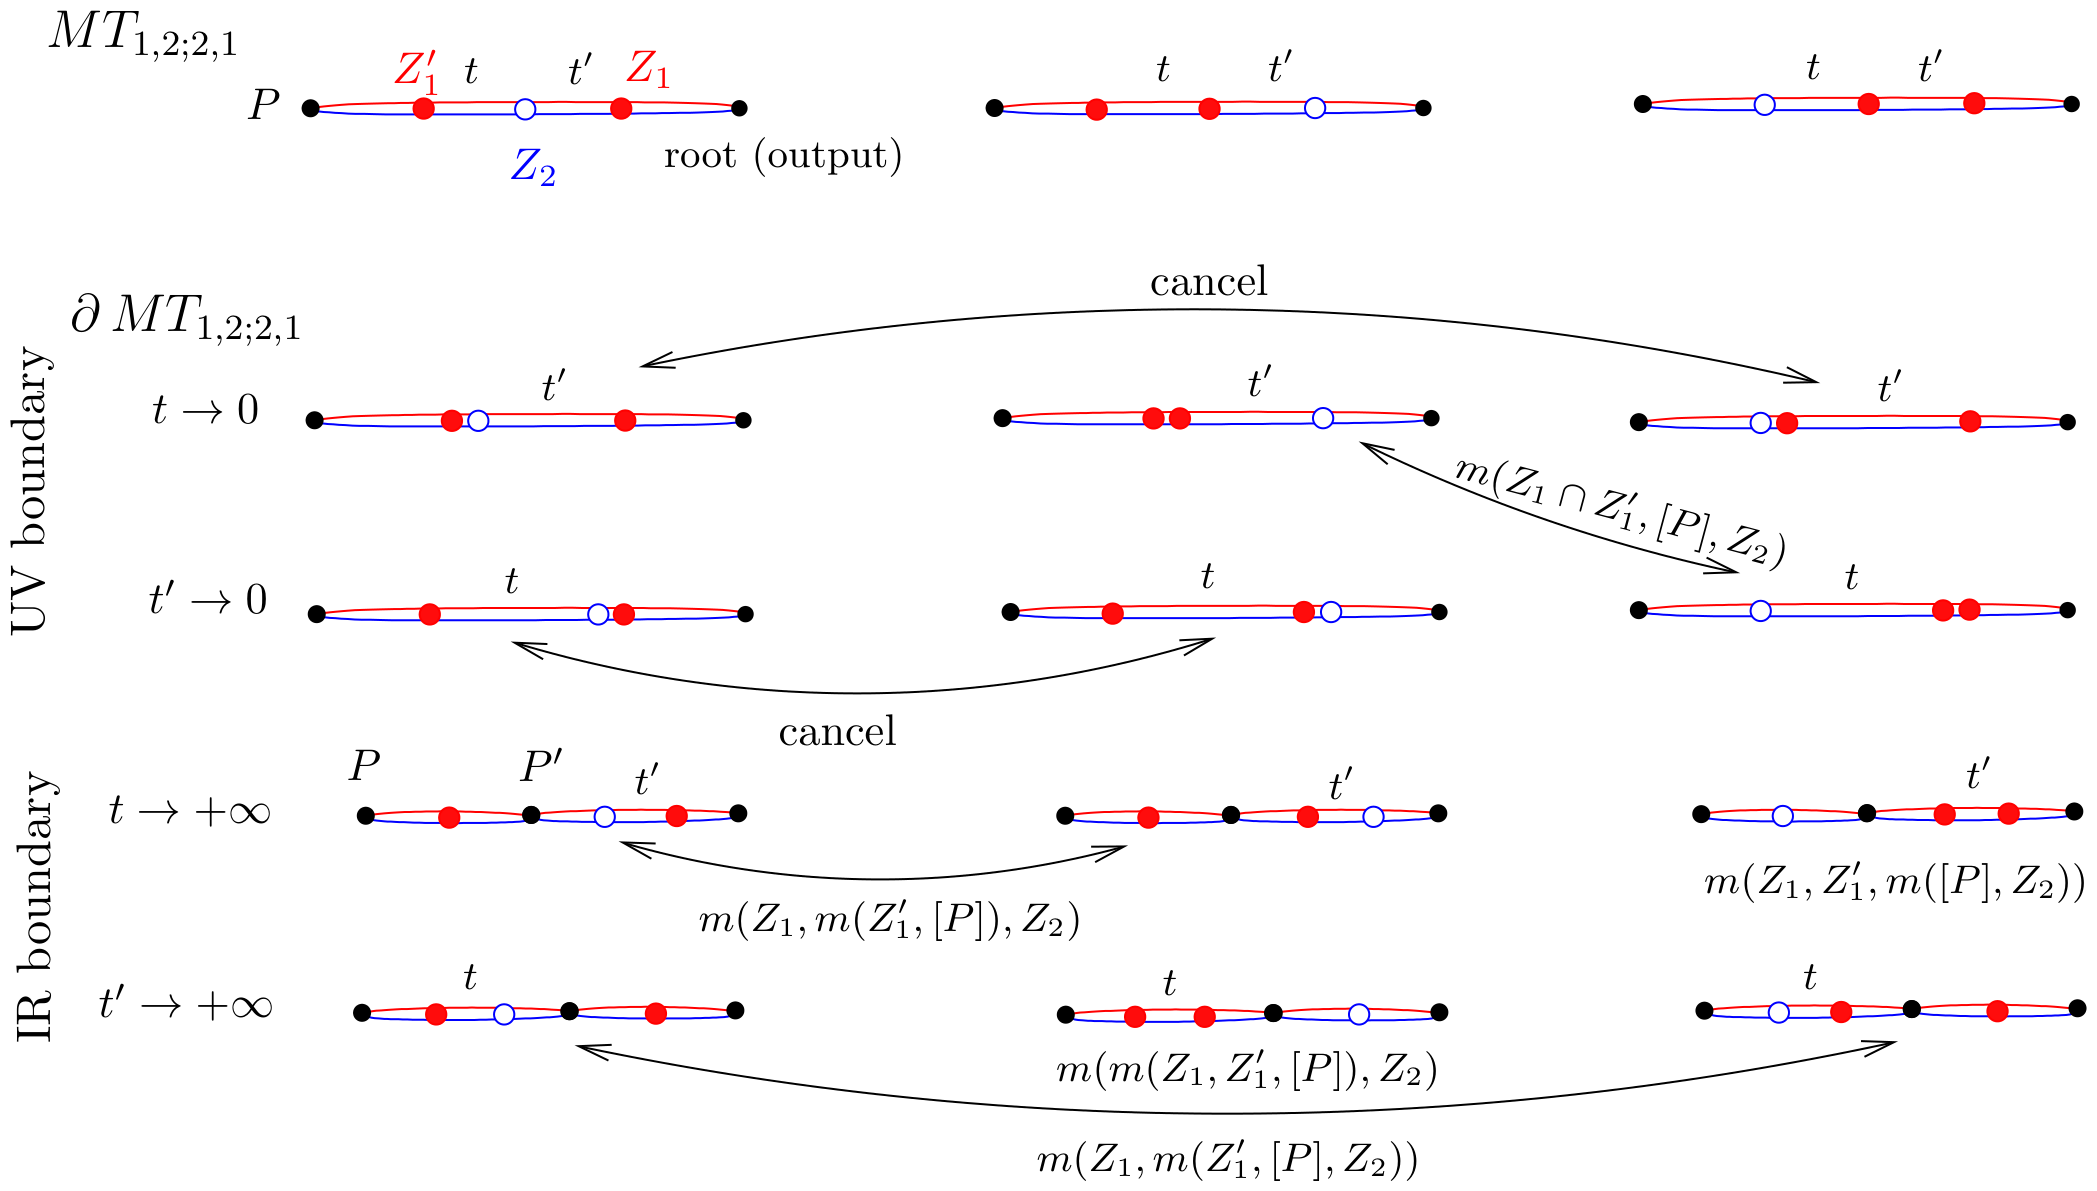
\includegraphics[width=0.98\linewidth]{fig12.png}
  \caption{度量树模空间的边界层片对 $\int_{\partial MT}I$（从而对 $A_\infty$ 关系式）的贡献。（原书 p.25）}
  \label{fig:12}
\end{figure}

\endinput
